\documentclass[twoside]{article}
\usepackage[a4paper]{geometry}
\geometry{verbose,tmargin=2.5cm,bmargin=2cm,lmargin=2cm,rmargin=2cm}
\usepackage{fancyhdr}
\pagestyle{fancy}

% nastavení pisma a~češtiny
\usepackage{lmodern}
\usepackage[T1]{fontenc}
\usepackage[utf8]{inputenc}
\usepackage[czech]{babel}

% odkazy
\usepackage{url}

\usepackage{float}
% vícesloupcové tabulky
\usepackage{multirow}
\usepackage{amssymb}
\usepackage{gensymb}
\usepackage{bbold}
\usepackage{amsmath}
\usepackage{mathtools}
\usepackage{commath}

% vnořené popisky obrázků
\usepackage{subcaption}

% automatická konverze EPS 
\usepackage{graphicx} 
\usepackage{epstopdf}
\epstopdfsetup{update}

\graphicspath{{./images}}

% odkazy a~záložky
\usepackage[unicode=true, bookmarks=true,bookmarksnumbered=true,
bookmarksopen=false, breaklinks=false,pdfborder={0 0 0},
pdfpagemode=UseNone,backref=false,colorlinks=true] {hyperref}

% Poznámky při překladu
\usepackage{xkeyval}	% Inline todonotes
\usepackage[textsize = footnotesize]{todonotes}
\presetkeys{todonotes}{inline}{}

%https://tex.stackexchange.com/questions/2783/bold-calligraphic-typeface
\DeclareMathAlphabet\mathbfcal{OMS}{cmsy}{b}{n}

% Zacni sekci slovem ukol
\renewcommand{\thesection}{Úkol \arabic{section}}
% enumerate zacina s pismenem
\renewcommand{\theenumi}{\alph{enumi}}

% smaz aktualni page layout
\fancyhf{}
% zahlavi
\usepackage{titling}
\fancyhf[HC]{\thetitle}
\fancyhf[HLE,HRO]{\theauthor}
\fancyhf[HRE,HLO]{\today}
 %zapati
\fancyhf[FLE,FRO]{\thepage}

% údaje o autorovi
\title{Automatické řízení: DÚ 8 -- Stavové metody}
\author{Vojtěch Michal}
\date{\today}

\begin{document}

\maketitle

\section{Model HIV - AIDS}
Nemoc AIDS dosud nedokážeme s jistotou plně vyléčit ani nedokážeme z těla pacienta úplně odstranit virus
HIV. Stále lépe ale dokážeme pomocí léků udržet počet částic viru v těle pacienta na nízké úrovni a tím
bránit vzniku nemoci AIDS.

Stavový model nákazy krevních buněk CD4+T, které virus HIV napadá, je po linearizaci v ekvilibriu
odpovídajícím bezpříznakovému pacientu dán rovnicemi

\begin{equation}
	\begin{split}
		\begin{bmatrix}
			\dot{T} \\
			\dot{T^{*}} \\
			\dot{\nu}
		\end{bmatrix} &= \underbrace{\begin{bmatrix}
			-004167 & 0 & -0.0058 \\
			0.0217 & -0.24 & 0.0058 \\
			0 & 100 & -2.4
		\end{bmatrix}}_{\mathbf{A}} \underbrace{\begin{bmatrix}
		T \\
		T^{*} \\
		\nu
	\end{bmatrix}}_{ \vec{x}} + \underbrace{\begin{bmatrix}
		5.2 \\
		-5.2 \\
		0
	\end{bmatrix}}_{\mathbf{B}} u \\
	y &= \underbrace{\begin{bmatrix}
		0 & 0 & 1
	\end{bmatrix}}_{\mathbf{C}} \begin{bmatrix}
		T \\
		T^{*} \\
		\nu
	\end{bmatrix}
\end{split}
\label{eq:zadani}
\end{equation}
Stavové veličiny $T$, $T^{*}$, $\nu$ jsou po řadě počet zdravých buněk, počet infikovaných buněk a počet volných
částic viru v krevním řečišti pacienta. Model zahrnuje léčbu pacienta pomocí léků RTI (inhibitory reverzní
transkriptázy) a tak je vstupem relativní dávkování RTI  $u \in [0,1]$ v rozsahu nulová až plná dávka. Výstupem
je počet volných částic viru.

Navrhněte řízení pomocí stavové zpětné vazby se specifikacemi: $e_{ss,step} = 0$, $OS\% = 10\%$, $T_s = 100~\text{dnů}$.
Přitom volte variantu zajišťující nulovou ustálenou odchylku robustně, tedy integrální řízení. \\
\\
\textbf{Řešení:}
V rovnici \eqref{eq:zadani} jsou pojmenovány jednotlivé matice stavového modelu pomocí standardního značení $\mathbf{A}$, $\mathbf{B}$, $\mathbf{C}$,
dále vektor stavů označíme $\vec{x}$. Nejprve se zaměřím na splnění požadavků na dynamiku systému ztělesněných v maximálním overshootu a době ustálení.

Samotná soustava má přenos
\begin{equation}
	G(s) = C (sI - A)^{-1} B =  \frac{-520(s+0.0200)}{(s+2.6433)(s+0.0192+0.0658i)(s+0.0192-0.0658i)}.
\end{equation}

\subsection{Požadavky na dynamiku}
Pomocí dvou požadavků se nám podaří umístit dva póly uzavřené smyčky, systém je ale zřejmě třetího řádu. Prozatím budu dynamiku 
navrhovat pro dominantní dvojici pólů -- tedy jakoby systém řádu 2 -- a třetím pólem zkusím později pokrátit nějakou nulu, nebo jej 
dám dostatečně daleko vlevo od dominantní dvojice. Zadaný maximální překmit CL nám určuje minimální damping ratio
\begin{equation}
	\zeta = \frac{- \text{ln}(OS\%/100)}{\sqrt{\pi^2 + \text{ln}^2(OS\%/100)}} = 0.5912.
\end{equation}
Pomocí relativního tlumení a požadovaného času ustálení pod dvě procenta lze vypočíst přirozenou frekvenci
\begin{equation}
	\omega_n =  -\frac{\text{ln}(0.02 \cdot \frac{\sqrt{1-\zeta^2}}{\zeta})}{\zeta \cdot T_s} = 0.0609~\text{rad} \cdot \text{den}^{-1} = 7.0506 \cdot 10^{-7} \text{rad} \cdot \text{s}^{-1}.
\end{equation}
Protože pro dominantní póly platí $Re(p) = \omega_n \zeta$ a $Im(p) = \omega_n \sqrt{1-\zeta^2}$, nalézají se v bodech 
\begin{equation}
	p_{1,2} = (-4.1682 \pm 5.6870i) \cdot 10^{-7}.
\end{equation}
Jejich vliv proto velmi výrazně (o pět dekád) dominuje nad vlivem nuly v bodě $z = -0.02$ a použití vzorců pro systém řádu 2 nezanáší do návrhu chybu.
Nulu $z$ pokrátíme posledním zbylým pólem. Cílem návrhu je dát uzavřené ZV smyčce charakteristický polynom
\begin{equation}
	c(s) = (s+4.1682 -5.6870i)(s + 4.1682 +5.6870i) \cdot \left(10^{-7}\right)^2 (s+0.02).
\end{equation}
Před hledáním regulátoru jsem ověřil, že $\text{rank}(\mathcal{C}) = \text{rank}(\mathbf{A})$ a systém je tedy úplně řiditelný.
Pro nalezení regulátoru použiji Ackermannův vzorec
\begin{equation}
	K = \begin{bmatrix}
		0 & 0 & 1
	\end{bmatrix} \mathcal{C}^{-1}  c(\mathbf{A}) = \begin{bmatrix}
		-0.0042 & 0.5077 & -0.0122
	\end{bmatrix},
\end{equation}
v němž figuruje inverze matice řiditelnosti $\mathcal{C}$ a dosazení matice systému $\mathbf{A}$ do žádaného char. polynomu $c(s)$.
Uzavřeném stavové zpětné vazby s regulátorem $K$ vytváří nový systém s maticí $A_{new} = A - BK$.
Na obrázku \ref{fig:wrong_gain} je výsledek simulace odezvy uzavřené smyčky na jednotkový skok.
\begin{figure}[htbp]
	\centering
	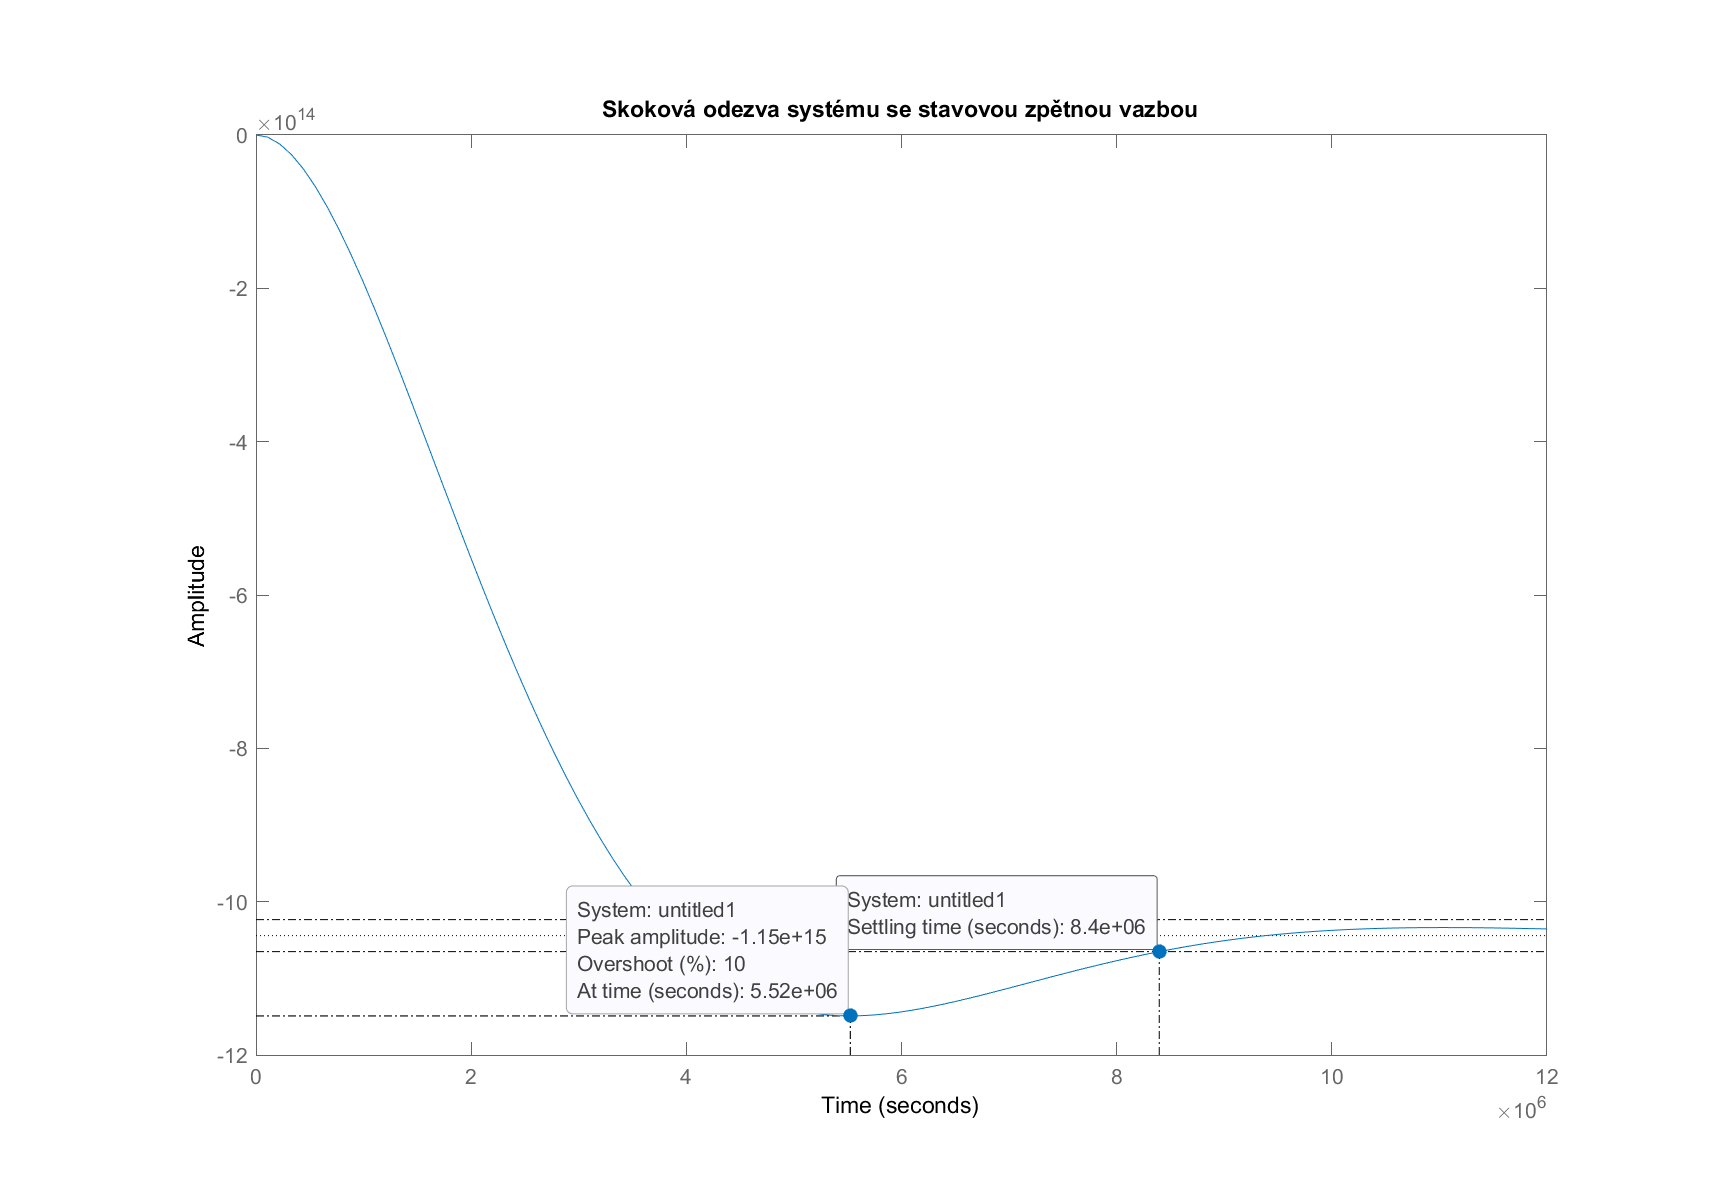
\includegraphics[width=\linewidth]{skokova_odezva.eps}
	\caption{Simulace odezvy soustavy po zavedení stavové zpětné vazby}
	\label{fig:wrong_gain}
\end{figure}
Překmit odezvy skutečně nepřesahuje 10\ a ustálení nastane po $100 \times 24 \times 3600 = 8640000$ sekundách.
Požadavky na dynamiku systému jsou splněny, jenom ta amplituda v řádu $10^{14}$ není v pořádku.

\subsection{Nastavení ustálené odchylky}
Uzavřená smyčka stavové zpětné vazby není schopna asymptoticky sledovat jednotkový skok. Použití feedforwardu pro nastavení
statického zesílení není přípustné s ohledem na robustnost, je tak nezbytné použít integrální řízení. Předraďme soustavě integrátor
a uzavřeme kolem celého seriového zapojení novou jednotkovou zpětnou vazbu. Vzniká systém řádu 4 s rovnicí


\begin{thebibliography}{9}

\bibitem{motivace}
	Robert H. Bishop, Supplementary lectures to book \emph{Modern control systems, 13th edition} 
		\url{https://youtu.be/uLeAot4Zrxo?t=13}

\end{thebibliography}



\end{document}

